% Part: sets-functions-relations
% Chapter: infinite
% Section: hilberts-hotel
%
\documentclass[../../../include/open-logic-section]{subfiles}

\begin{document}

\olfileid{sfr}{infinite}{hilbert}
\olsection{Hotel Hilbert}

Himpunan wilangan natural mesthi katon tanpa wates. Mula, yen kita ora
arep \emph{langsung nganggep} wilangan natural wis ana, langkah
kapisan kudu njlentrehake himpunan tanpa wates nganggo istilah kang ora
mbutuhake panyebutan wilangan natural iku dhewe. Iki salah siji cara
kang becik, kang diandharake Hilbert ing kuliah taun 1924. Dheweke
njaluk kita mbayangake
\begin{quote}
[\ldots] hotel kang kamare winates cacahe. Saben kamar kudu dienggoni
pas siji tamu. Yen para tamu banjur ijol kamar kanthi sawenehing cara,
[nanging] saben kamar tetep ora dienggoni luwih saka siji wong, ora
ana kamar kang dadi kosong, lan kanthi cara iki sing duwe hotel ora
bisa nyawisake panggonan anyar kanggo tamu kang mentas teka [\ldots
\textparagraph \ldots]

Saiki kita netepake yen hotel mau duwe kamar tanpa wates cacahe kang
diwenehi nomer $1$, $2$, $3$, $4$, $5$, \dots, lan saben kamar
dienggoni pas siji tamu. Sanalika ana tamu anyar teka, sing duwe hotel
mung perlu mindhah saben tamu lawas menyang kamar kanthi nomer siji
luwih gedhe, lan kamar~$1$ bakal kosong kanggo tamu kang mentas teka.
	\begin{center}
		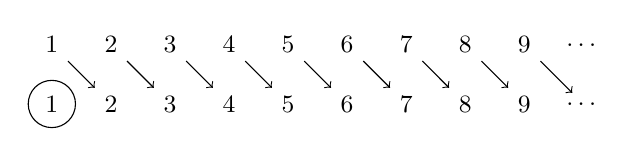
\begin{tikzpicture}[scale = .75]
		\foreach \x in {1, 2, 3, 4, 5, 6, 7, 8, 9}
		{
			\node (\x a) at (\x, 1) {\small{\x}};
			\node (\x b) at (\x, 2) {\small{\x}};
		}
		\node (dotsa) at (10, 1) {\small{\ldots}};
		\node (dotsb) at (10, 2) {\small{\ldots}};
		\draw[->] (1b)--(2a);
		\draw[->] (2b)--(3a);
		\draw[->] (3b)--(4a);
		\draw[->] (4b)--(5a);
		\draw[->] (5b)--(6a);
		\draw[->] (6b)--(7a);
		\draw[->] (7b)--(8a);
		\draw[->] (8b)--(9a);
		\draw[->] (9b)--(dotsa);
		\draw (1,1) circle (.4);
		\end{tikzpicture}
	\end{center}
	(diterbitake ing \citealt[730]{EwaldSieg2013}; terjemahan kita)
\end{quote}
Bab kang wigati yaiku Hotel Hilbert duwe kamar tanpa wates cacahe; lan
andharane bisa kita gunakake kanggo nemtokake apa tegese pratelan iku.
Pancen, iki uga cara Dedekind (mesthi wae diandharake ing kene nganggo
anakronisme kang gedhe banget; definisi Dedekind asale saka
\citeyear{Dedekind1888}):

\begin{defn}\ollabel{defn:DedekindInfinite}
Himpunan $A$ iku \emph{tanpa wates miturut Dedekind} yen lan mung yen
ana !!a{injection} saka~$A$ menyang subhimpunan sejati saka~$A$. Yaiku,
ana $o \in A$ lan !!a{injection} $f \colon A \to A$ saengga
$o \notin \ran{f}$.
\end{defn}

\end{document}
